\subsubsection{Cross-Asset Dependence Models: Derivations and Diagnostics (Pipeline~B)}
\label{sec:cross_asset_supp}

This appendix provides the technical background for the SIM and copula constructions used in Section~\ref{sec:cross_asset} of the main text. These constructions constitute \emph{Pipeline~B}: per-asset marginals come from the independent CHMMs of Pipeline~A (Section~\ref{sec:cross_asset_univariate}) and joint dependence is overlaid on top. Pipeline~A stays purely univariate; Pipeline~B is the sole multi-asset pipeline in the paper.

\paragraph{Sklar's theorem and the rank-reordering simulator.}
Sklar's theorem \cite{sklar1959fonctions, nelsen2006introduction} states that any $d$-dimensional joint CDF $H(g_1, \dots, g_d)$ with continuous marginals $F_1, \dots, F_d$ can be written as $H = C(F_1, \dots, F_d)$ for a unique copula $C$.
The rank-reordering simulator exploits this uniqueness.
If $\tilde{\mathbf{G}}$ is a matrix whose $j$-th column is an i.i.d.\ sample from $F_j$, and $\mathbf{U}$ is an independent sample from $C$, then reordering each column of $\tilde{\mathbf{G}}$ so that its ranks match $\mathbf{U}$'s produces a sample from $H$, up to discrete approximation error in the empirical ranks.
Crucially, reordering never creates new values: each column of the output is a permutation of the corresponding column of $\tilde{\mathbf{G}}$, so marginal distributions are preserved exactly \cite{iman1982distribution}.

\paragraph{Kendall's $\tau$ inversion.}
Given IS returns $\mathbf{R} \in \mathbb{R}^{T \times d}$, we estimate the pairwise Kendall's $\tau_{ij}$ from concordant/discordant pair counts and invert to the correlation scale via the analytic relationship $\rho_{ij} = \sin(\pi \tau_{ij} / 2)$, which holds exactly for the Gaussian copula family and is commonly used as a robust correlation estimator for the Student-t copula \cite{embrechts2002correlation, mcneil2015quantitative}.
The resulting matrix $\hat{\Sigma}$ is symmetric but not guaranteed positive semi-definite; we project to the nearest PSD matrix by clipping negative eigenvalues to $10^{-8}$ and rescaling the diagonal to unity.

\paragraph{Profile MLE for $\nu$.}
The Student-t copula log-density at a single pseudo-uniform observation $\mathbf{u} \in [0,1]^d$, with $x_j = t_\nu^{-1}(u_j)$ and $\mathbf{x} = (x_1, \dots, x_d)^\top$, is
\begin{align}
    \log c_t(\mathbf{u}; \Sigma, \nu)
    \;=\;&
    \log \Gamma\!\left(\tfrac{\nu+d}{2}\right)
    + (d-1)\,\log \Gamma\!\left(\tfrac{\nu}{2}\right)
    - d\,\log \Gamma\!\left(\tfrac{\nu+1}{2}\right)
    - \tfrac{1}{2} \log |\Sigma|
    \notag \\
    &\;
    - \tfrac{\nu+d}{2}\,\log\!\left(1 + \tfrac{\mathbf{x}^{\!\top} \Sigma^{-1} \mathbf{x}}{\nu}\right)
    + \sum_{j=1}^{d} \tfrac{\nu+1}{2}\,\log\!\left(1 + \tfrac{x_j^2}{\nu}\right).
    \label{eq:tcop_ll}
\end{align}
Summing over $t = 1, \dots, T$ pseudo-observations yields the profile log-likelihood as a function of $\nu$ with $\Sigma$ held fixed at the Kendall's-$\tau$ estimate.
We evaluate equation~\eqref{eq:tcop_ll} on the discrete grid $\nu \in \{2, 3, 4, 5, 6, 8, 10, 15, 20, 30\}$ and select $\hat{\nu}$ as the grid point with the largest total log-likelihood.
In Section~\ref{sec:cross_asset} the selected value was $\hat{\nu} = 6$ on the six-asset universe.

\paragraph{Sampling the copula.}
To sample $T$ rows from the $d$-dimensional Gaussian copula with correlation $\Sigma$, we (i) compute the Cholesky factor $\Sigma = L L^\top$, (ii) draw $Z \sim \mathcal{N}(0, I_d)$ i.i.d.\ and form $Y = L Z$, and (iii) return $U = \Phi(Y)$ componentwise.
For the Student-t copula with degrees of freedom $\nu$, we draw $W \sim \chi^2_\nu / \nu$ independent of $Y$ and form the multivariate-$t$ variate $X = Y / \sqrt{W}$, then return $U = t_\nu(X)$ componentwise.

\paragraph{SIM regression summary.}
Table~\ref{tab:sim_regression} reports the fitted SIM regression coefficients and goodness-of-fit statistics for the non-market assets in Section~\ref{sec:cross_asset}.
QQQ's high $R^2 = 0.840$ reflects that the Nasdaq-100 ETF is essentially a linear combination of large-cap technology names that also drive the S\&P~500 index, while JNJ's lower $R^2 = 0.260$ reflects the limited systematic exposure of low-beta healthcare stocks.
These factor loadings and residual magnitudes are what the SIM simulation re-injects at simulation time, and they explain the uneven per-asset KS pass rates reported in Table~\ref{tab:cross_asset_supp_summary}.

\begin{table}[H]
\centering
\caption{SIM regression $\hat{G}_{j,t} = \hat{\alpha}_j + \hat{\beta}_j G_{\text{SPY},t} + \hat{\eta}_{j,t}$ for the five non-market assets, fitted on the $2014$-$01$-$03$ through $2024$-$01$-$03$ IS window ($T = 2{,}516$).}
\label{tab:sim_regression}
\small
\begin{tabular}{l ccc}
\toprule
Ticker & $\hat{\alpha}$ & $\hat{\beta}$ & $R^2$ \\
\midrule
NVDA & $0.321$   & $1.694$ & $0.371$ \\
JNJ  & $0.002$   & $0.576$ & $0.260$ \\
JPM  & $-0.008$  & $1.223$ & $0.507$ \\
AAPL & $0.111$   & $1.205$ & $0.492$ \\
QQQ  & $0.047$   & $1.122$ & $0.840$ \\
\bottomrule
\end{tabular}
\end{table}

\subsubsection{Student-t Copula Profile Log-Likelihood (Pipeline~B)}
\label{sec:copula_profile_supp}

Figure~\ref{fig:copula_profile} plots the profile log-likelihood of the Student-t copula used inside Pipeline~B, computed on the six-asset SPY cross-section over the grid $\nu \in \{2, 3, 4, 5, 6, 8, 10, 15, 20, 30\}$ used in Section~\ref{sec:cross_asset}.
The curve is smooth and single-peaked, with $\nu^{*} = 6$ attaining the maximum profile log-likelihood ($6157.47$), and the neighbouring grid points $\nu = 5$ ($6143.37$) and $\nu = 8$ ($6148.37$) each within $15$ profile-log-likelihood units of the peak, indicating a shallow-but-clean optimum that agrees with the $4$--$10$ range typically reported for equity-portfolio Student-t copulas in the risk-management literature.

\begin{figure}[h]
\centering
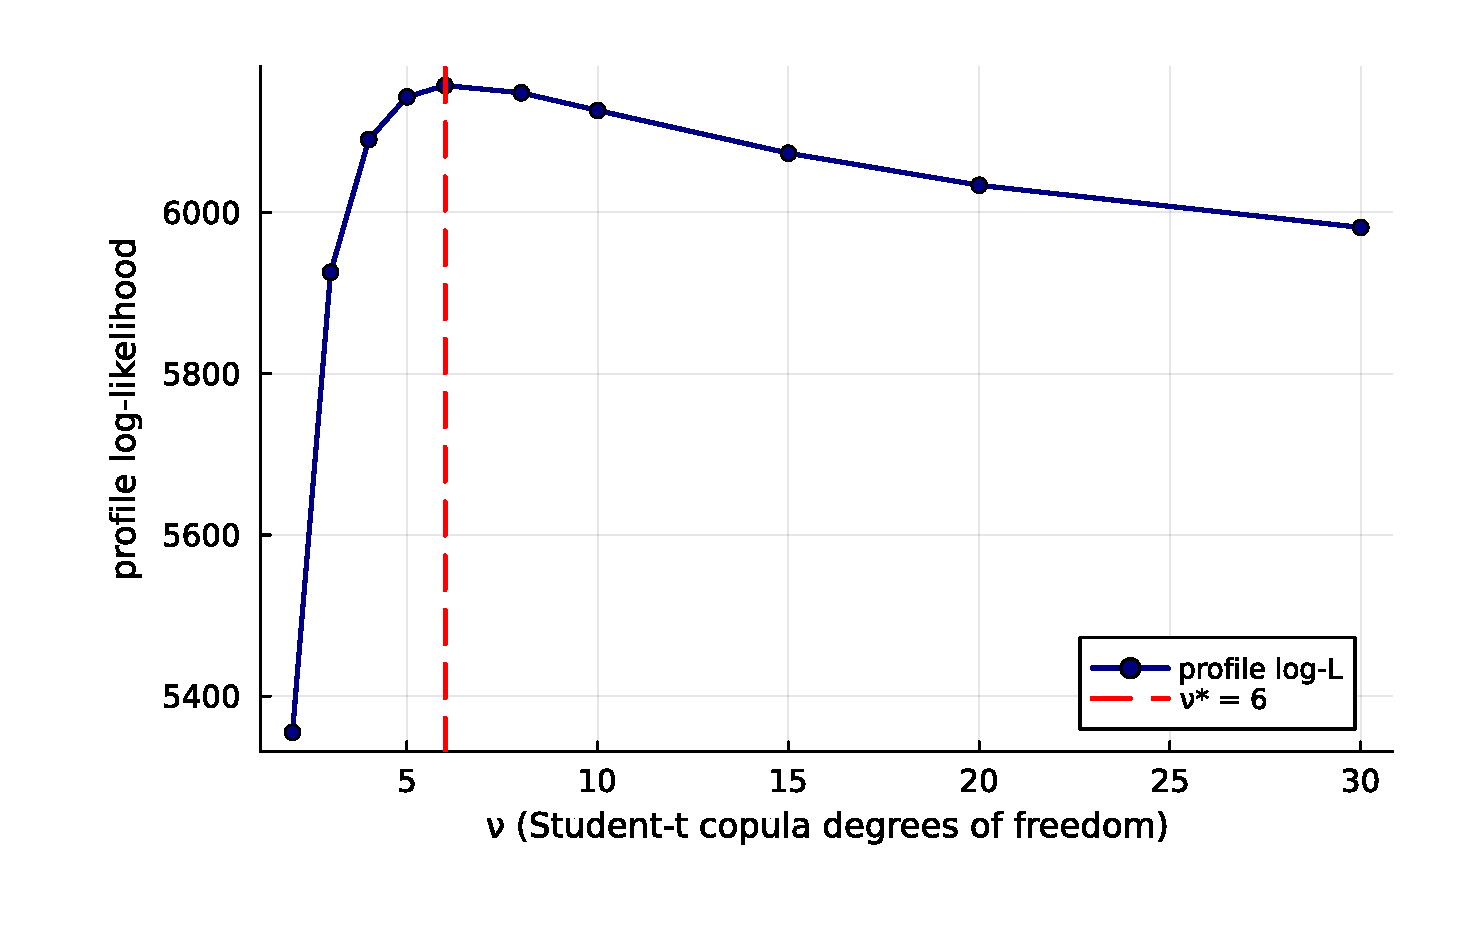
\includegraphics[width=0.70\textwidth]{figs/Fig-Copula-Profile.pdf}
\caption{\textbf{Profile log-likelihood of the Student-t copula} used inside Pipeline~B on the six-asset SPY cross-section (SPY, NVDA, JNJ, JPM, AAPL, QQQ; IS window 2014-01-03 through 2024-01-03). The vertical axis is the profile log-likelihood evaluated at each degrees-of-freedom value $\nu$ on the grid $\{2, 3, 4, 5, 6, 8, 10, 15, 20, 30\}$; the dashed red line marks the profile MLE $\nu^{*} = 6$ (peak value 6157.47). The CHMM-N marginals are held fixed at the Pipeline~A per-asset fits while $\nu$ is varied.}
\label{fig:copula_profile}
\end{figure}

\subsubsection{Cross-Asset Correlation Heat Maps (Pipeline~B, Companion to Table~\ref{tab:cross_asset_supp_summary})}
\label{sec:cross_asset_corr_supp}

Figure~\ref{fig:cross_asset_corr} visualises the observed and path-averaged simulated correlation matrices for the dependence models of Section~\ref{sec:cross_asset}.
The panel ordering is SIM, Gaussian copula, Student-t copula (each reported quantitatively in Table~\ref{tab:cross_asset_supp_summary}), plus a truncated C-vine variant with SPY as root for visual comparison.
All five panels share the six-asset SPY cross-section and the same CHMM-N marginals at $K = 18$, so any visible differences between the simulated panels reflect only the dependence construction.

\begin{figure}[H]
\centering
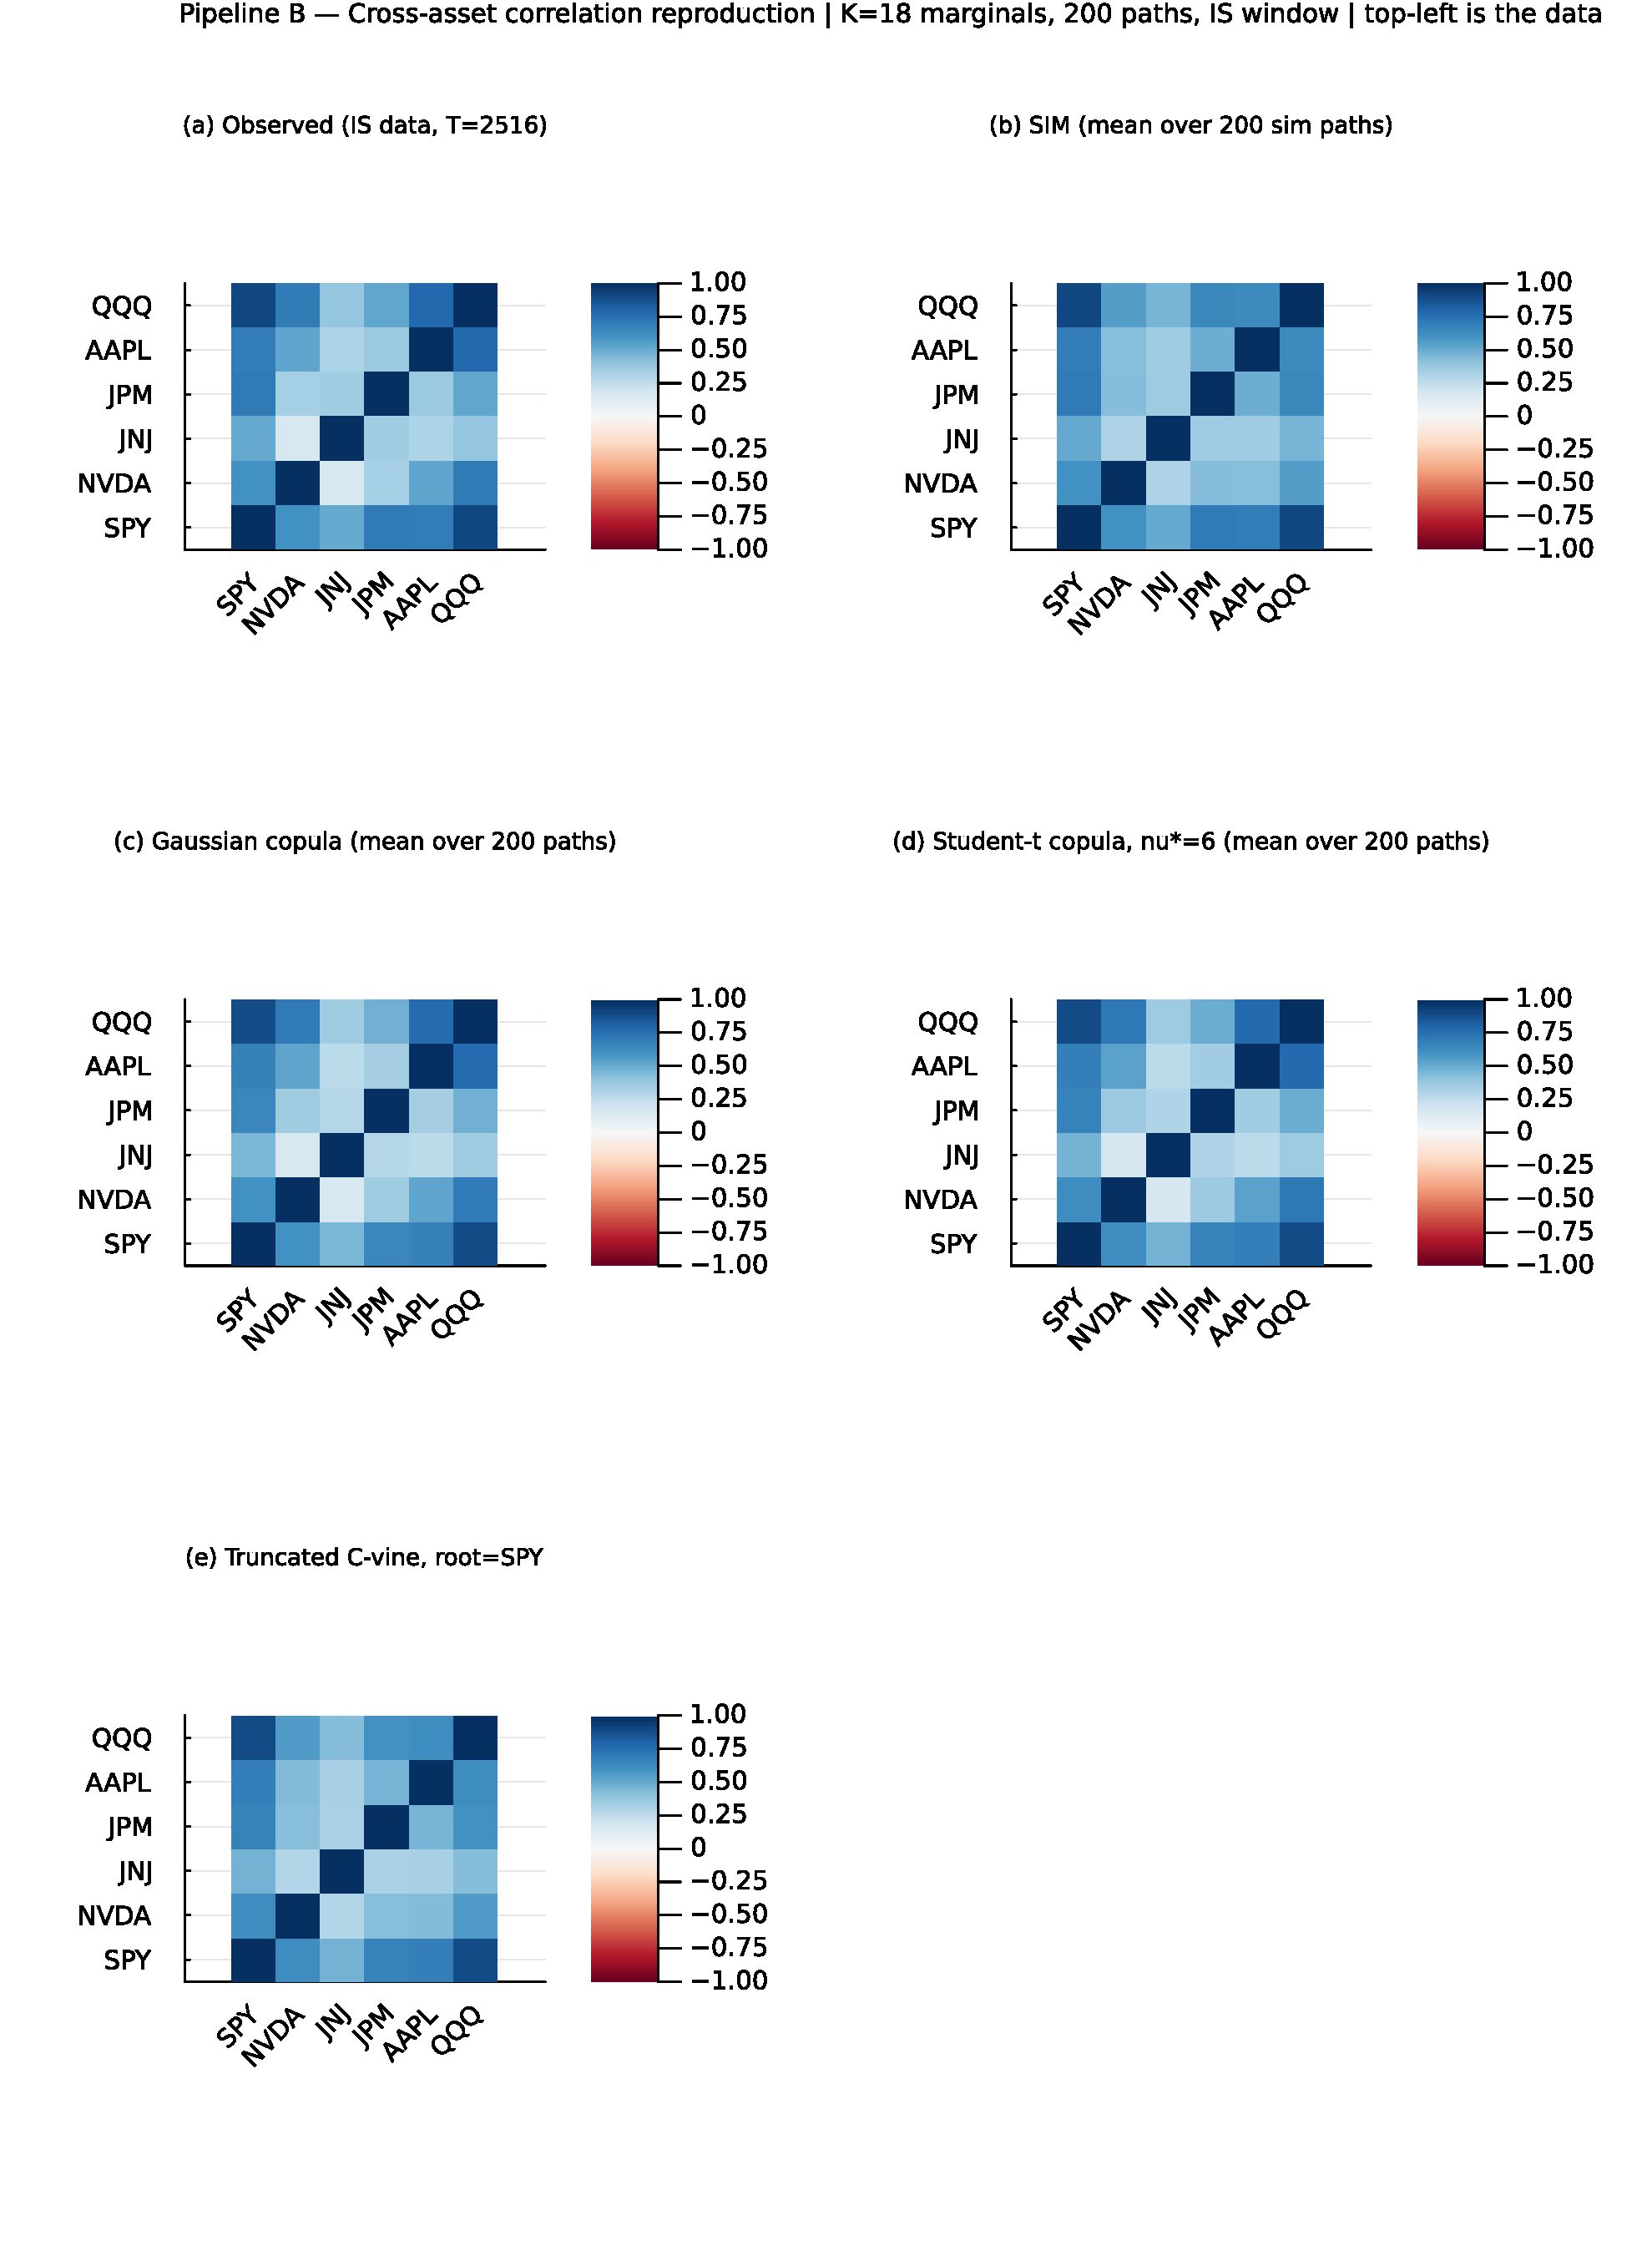
\includegraphics[width=0.75\textwidth]{figs/Fig-Cross-Asset-Correlation.pdf}
\caption{\textbf{Cross-asset IS correlation reproduction across dependence models} (Pipeline~B, companion to Table~\ref{tab:cross_asset_supp_summary}). Panel~(a), top-left: \emph{observed} correlation matrix on 2014-01-03 through 2024-01-03 daily excess log returns for SPY, NVDA, JNJ, JPM, AAPL, QQQ (IS window, $T_{\text{IS}} = 2{,}516$). Panel~(b), top-right: path-averaged correlation under the Single Index Model with SPY as market factor. Panel~(c), middle-left: path-averaged correlation under the Gaussian copula on CHMM marginals. Panel~(d), middle-right: path-averaged correlation under the Student-t copula on CHMM marginals, $\nu^* = 6$. Panel~(e), bottom-left: path-averaged correlation under a truncated C-vine copula with SPY as root. Each simulated panel averages over 200 paths of length $T_{\text{IS}}$. All marginals are the per-asset CHMM-N fits at $K = 18$ from Table~\ref{tab:cross_asset}; color scale in $[-1, 1]$, red-white-blue (RdBu) diverging. Closer visual match to panel~(a) is better.}
\label{fig:cross_asset_corr}
\end{figure}

\subsubsection{Non-US Asset Class Extension and Per-Pair OoS Off-Diagonal Breakdown}
\label{sec:non_us_asset_supp}

The body universe (SPY, NVDA, JNJ, JPM, AAPL, QQQ) is six US-listed equity tickers from one country-index family. To probe whether the cross-asset construction generalises off the equity cluster we extend the universe with GLD (SPDR Gold Trust), a US-listed ETF whose underlying is physically-backed gold, i.e.\ a non-equity commodity asset class.

\paragraph{GLD Pipeline-A univariate fidelity.}
Fitting CHMM-N, CHMM-t, and CHMM-L on the GLD return series at $K = 18$ produces $100\%$ IS KS pass rate for all three families and observed IS excess kurtosis $3.6$ matched closely by CHMM-L ($2.2$); on OoS, however, the KS pass rate collapses to $0\%$ for all three families against an observed OoS excess kurtosis of $6.5$. Inspection of the GLD price path on the $2024$--$2026$ OoS window shows the asset re-priced from $\sim 200$ to $\sim 300$ on a persistent demand shock not represented in the $2014$--$2024$ IS regime library. This is the same stationarity-scope artefact as the NVDA / JPM single-name OoS cliffs reported in Section~\ref{sec:cross_asset_univariate}, on a non-equity asset; the limitation is not equity-specific.

\paragraph{Pipeline-B: 7-ticker Student-t copula off-diagonal MAE.}
Refitting the Student-t copula on the augmented seven-ticker universe at $\nu^\star = 6$ gives IS off-diagonal MAE of $0.029$ (six-ticker baseline: $0.027$) and OoS off-diagonal MAE of $0.179$ (six-ticker baseline: $0.211$). Adding the low-equity-correlation gold ETF \emph{reduces} the OoS off-diagonal MAE, because the equity-cluster correlation degradation is the dominant component; pairs involving GLD have moderate IS-to-OoS shifts ($|\Delta| \in [0.04, 0.19]$) while the largest equity-cluster pairs (JNJ-QQQ, SPY-JNJ, NVDA-JNJ) have $|\Delta| > 0.48$ on OoS.

\paragraph{Per-pair OoS gap localisation.}
Table~\ref{tab:per_pair_offdiag_mae} reports the per-pair off-diagonal absolute deviation between observed and path-averaged simulated correlation matrices on IS and OoS, sorted by OoS $|\Delta|$. The OoS gap concentrates in pairs involving JNJ (the defensive single-name proxy): JNJ's IS correlation with the broad equity factor (QQQ, SPY) collapses on OoS, in some pairs flipping sign, and the IS-fixed copula has no mechanism for tracking that shift. The gold-ETF pairs (SPY-GLD, JPM-GLD, JNJ-GLD, QQQ-GLD) sit in the middle of the ranking with $|\Delta|$ between $0.10$ and $0.19$ on OoS. The dominant cause of the OoS off-diagonal gap is therefore neither equity-cluster size nor copula-degree mis-specification but a single-name regime shift in the JNJ-equity-factor relationship that the IS-fitted dependence layer cannot anticipate.

\begin{table}[t]
\centering
\small
\caption{\textbf{Per-pair off-diagonal correlation MAE on the seven-ticker universe} (Pipeline B, Student-t copula on CHMM-N marginals at $K = 18$, $200$ paths, $\nu^\star = 6$). For each ticker pair $(i, j)$ the table reports $|\Sigma_{\text{sim,avg}}[i,j] - \Sigma_{\text{obs}}[i,j]|$ on IS and OoS, ranked by OoS $|\Delta|$. Only the ten largest-OoS-gap pairs are shown for compactness.}
\label{tab:per_pair_offdiag_mae}
\begin{tabular}{l c c c}
\toprule
Pair & IS $|\Delta|$ & OoS $|\Delta|$ & OoS $-$ IS \\
\midrule
JNJ-QQQ   & $0.027$ & $0.544$ & $0.517$ \\
SPY-JNJ   & $0.037$ & $0.509$ & $0.473$ \\
NVDA-JNJ  & $0.017$ & $0.489$ & $0.473$ \\
NVDA-AAPL & $0.011$ & $0.278$ & $0.268$ \\
JNJ-JPM   & $0.046$ & $0.261$ & $0.216$ \\
JNJ-AAPL  & $0.042$ & $0.244$ & $0.202$ \\
AAPL-QQQ  & $0.003$ & $0.227$ & $0.224$ \\
JPM-GLD   & $0.027$ & $0.187$ & $0.160$ \\
SPY-GLD   & $0.038$ & $0.127$ & $0.089$ \\
JNJ-GLD   & $0.015$ & $0.117$ & $0.101$ \\
\bottomrule
\end{tabular}
\end{table}


